\pdfminorversion=4
\documentclass[aspectratio=169]{beamer}

\mode<presentation>
{
  \usetheme{default}
  \usecolortheme{default}
  \usefonttheme{default}
  \setbeamertemplate{navigation symbols}{}
  \setbeamertemplate{caption}[numbered]
  \setbeamertemplate{footline}[frame number]  % or "page number"
  \setbeamercolor{frametitle}{fg=white}
  \setbeamercolor{footline}{fg=black}
} 

\usepackage[english]{babel}
\usepackage[utf8x]{inputenc}
\usepackage{tikz}
\usepackage{courier}
\usepackage{array}
\usepackage{bold-extra}
\usepackage{minted}
\usepackage[thicklines]{cancel}
\usepackage{fancyvrb}

\xdefinecolor{dianablue}{rgb}{0.18,0.24,0.31}
\xdefinecolor{darkblue}{rgb}{0.1,0.1,0.7}
\xdefinecolor{darkgreen}{rgb}{0,0.5,0}
\xdefinecolor{darkgrey}{rgb}{0.35,0.35,0.35}
\xdefinecolor{darkorange}{rgb}{0.8,0.5,0}
\xdefinecolor{darkred}{rgb}{0.7,0,0}
\definecolor{darkgreen}{rgb}{0,0.6,0}
\definecolor{mauve}{rgb}{0.58,0,0.82}

\title[2019-11-07-chep-awkward]{Alexander and the Ragged, Jagged, \\ Nested, Indirected, Very Awkward Arrays}
\author{\underline{Jim Pivarski}, David Lange, Peter Elmer}
\institute{Princeton University -- IRIS-HEP}
\date{November 7, 2019}

\usetikzlibrary{shapes.callouts}

\begin{document}

\logo{\pgfputat{\pgfxy(0.11, 7.4)}{\pgfbox[right,base]{\tikz{\filldraw[fill=dianablue, draw=none] (0 cm, 0 cm) rectangle (50 cm, 1 cm);}\mbox{\hspace{-8 cm}
\includegraphics[height=1 cm]{princeton-logo-long.png}\hspace{0.1 cm}\raisebox{0.1 cm}{
\includegraphics[height=0.8 cm]{iris-hep-logo-long.png}}\hspace{0.1 cm}}}}}

\begin{frame}
  \titlepage

\vspace{-3.5 cm}
\hfill 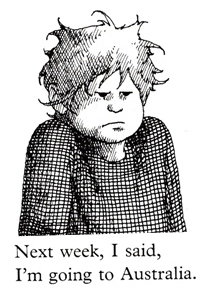
\includegraphics[height=4.5 cm]{alexander.png}
\vspace{-1 cm}
\end{frame}

\logo{\pgfputat{\pgfxy(0.11, 7.4)}{\pgfbox[right,base]{\tikz{\filldraw[fill=dianablue, draw=none] (0 cm, 0 cm) rectangle (50 cm, 1 cm);}\mbox{\hspace{-8 cm}
\includegraphics[height=1 cm]{princeton-logo.png}\hspace{0.1 cm}\raisebox{0.1 cm}{
\includegraphics[height=0.8 cm]{iris-hep-logo.png}}\hspace{0.1 cm}}}}}

% Uncomment these lines for an automatically generated outline.
%\begin{frame}{Outline}
%  \tableofcontents
%\end{frame}

% START START START START START START START START START START START START START

\begin{frame}{After reconstruction, physics analyzers need\ldots}
\Large

\begin{columns}
\column{0.5\linewidth}
\begin{center}
\textcolor{darkblue}{\LARGE rich data structures}
\end{center}

A general programming language like C++ or Python provides this, though C++ is hard to use for data analysis and Python is slow.

\column{0.5\linewidth}
\begin{uncoverenv}<2->
\begin{center}
\textcolor{darkblue}{\LARGE interactivity}
\end{center}

Data-oriented DSLs like NumPy and Pandas are convenient, but only for simple data: rectilinear arrays of numbers.
\end{uncoverenv}
\end{columns}

\vspace{0.25 cm}
\begin{columns}
\column{0.5\linewidth}
\begin{uncoverenv}<3->
\begin{center}
\textcolor{darkblue}{\LARGE speed}
\end{center}

Results should pop up quickly enough that you don't lose your train of thought.
\end{uncoverenv}
\end{columns}
\end{frame}

\begin{frame}{Composable, vectorization-friendly data structures}
\large
\vspace{0.25 cm}
\begin{center}
\only<1>{An array of variable-length arrays (``ragged'' or ``jagged'') can be built out of flattened contents and offsets specifying the beginning of each subarray.}\only<2>{Multiple levels of variable-length arrays (``doubly jagged'') can be built by using one jagged array as the content of the other.}\only<3>{More complex data structures can be built by adding columnar components, such as records with named fields, mixed data types, pointers, lazy loading\ldots}
\end{center}

\vspace{-0.25 cm}
\begin{columns}
\column{1.15\linewidth}
\only<1>{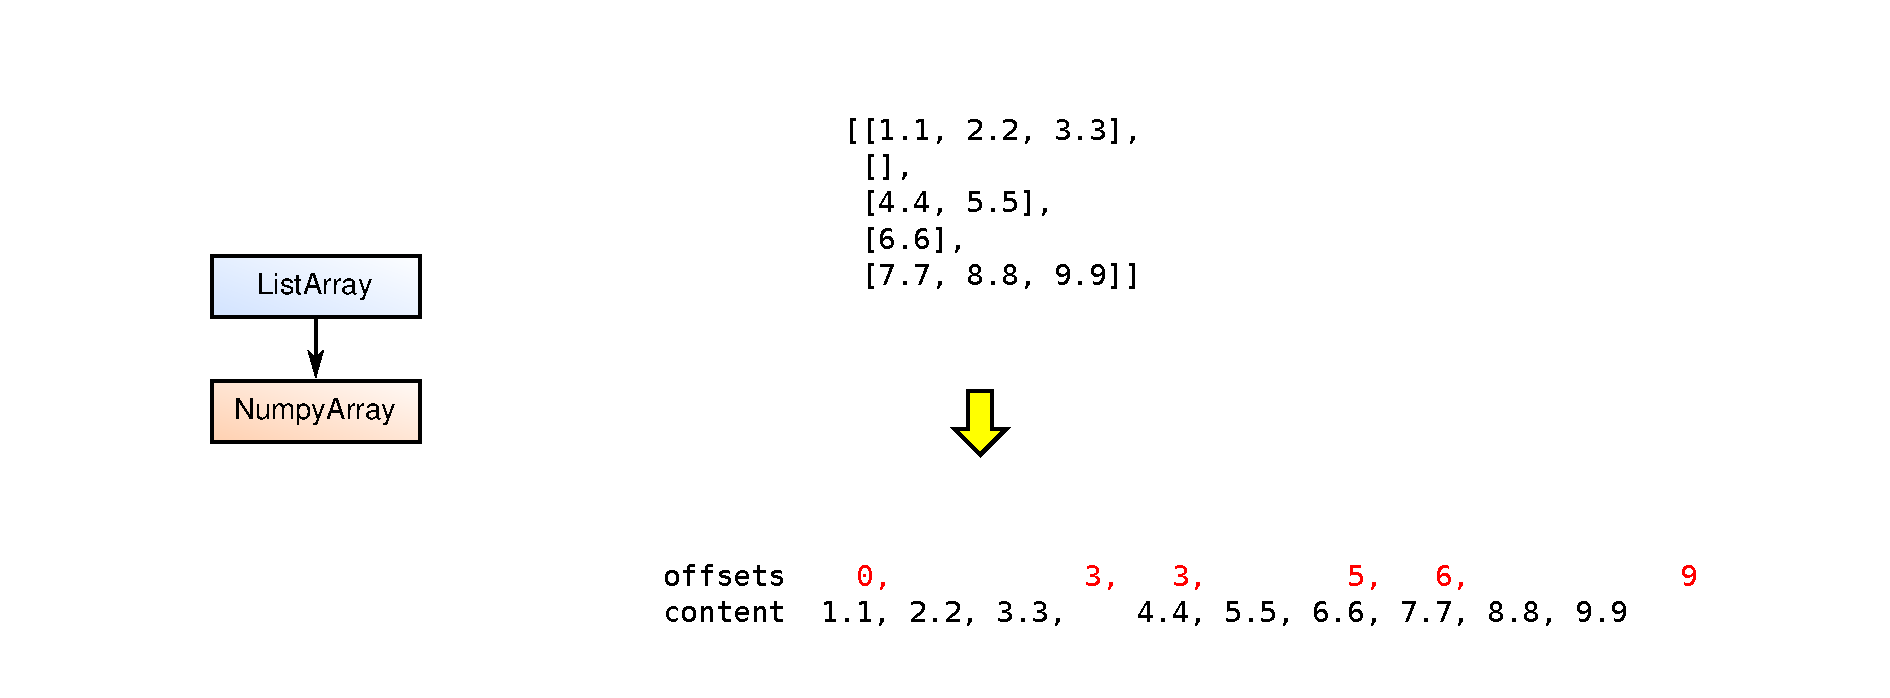
\includegraphics[width=\linewidth]{composable-1.pdf}}\only<2>{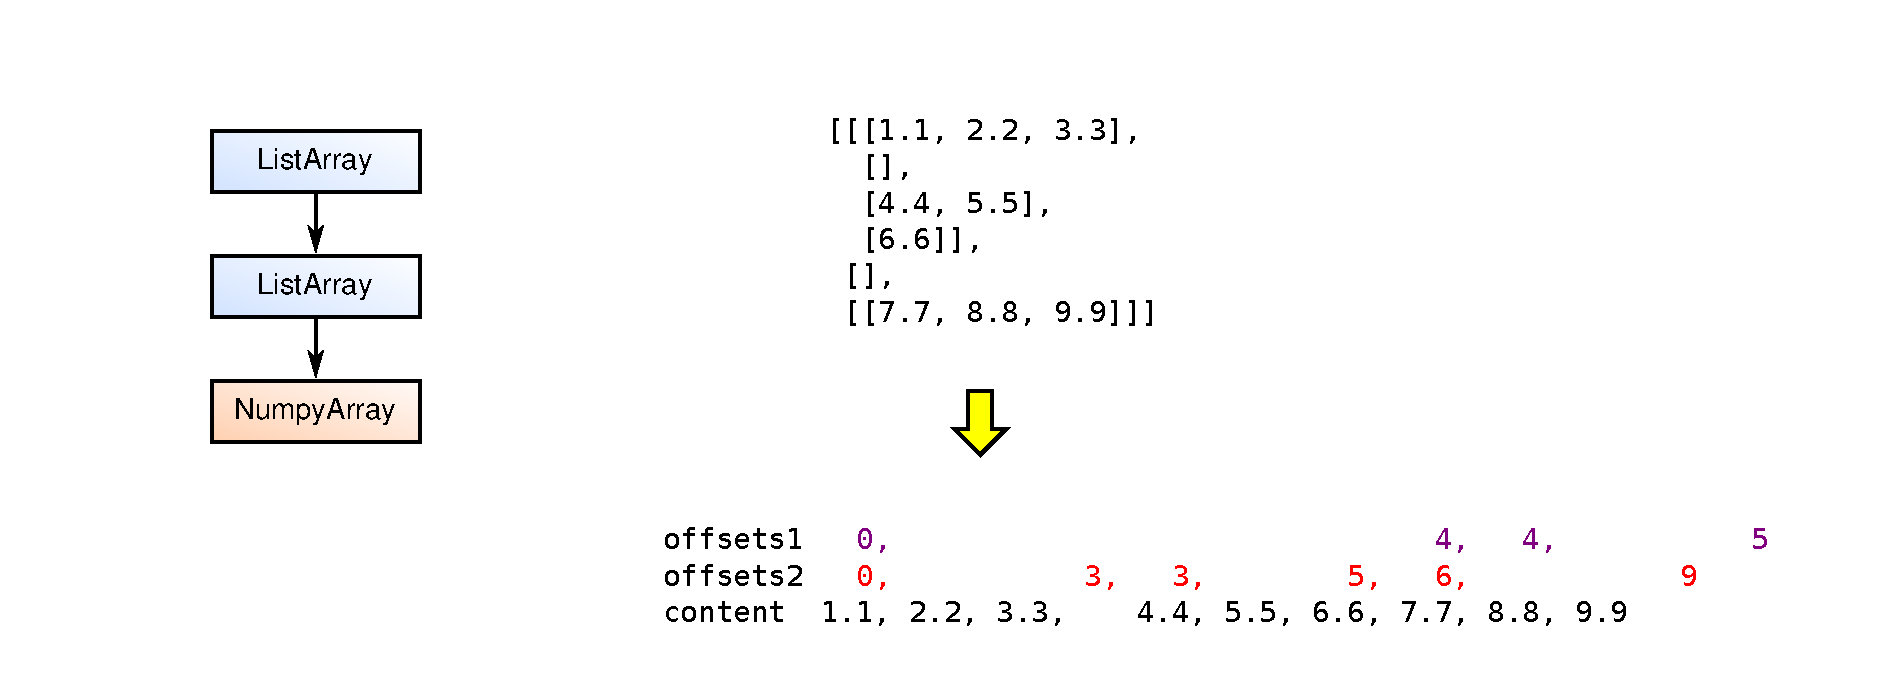
\includegraphics[width=\linewidth]{composable-2.pdf}}\only<3>{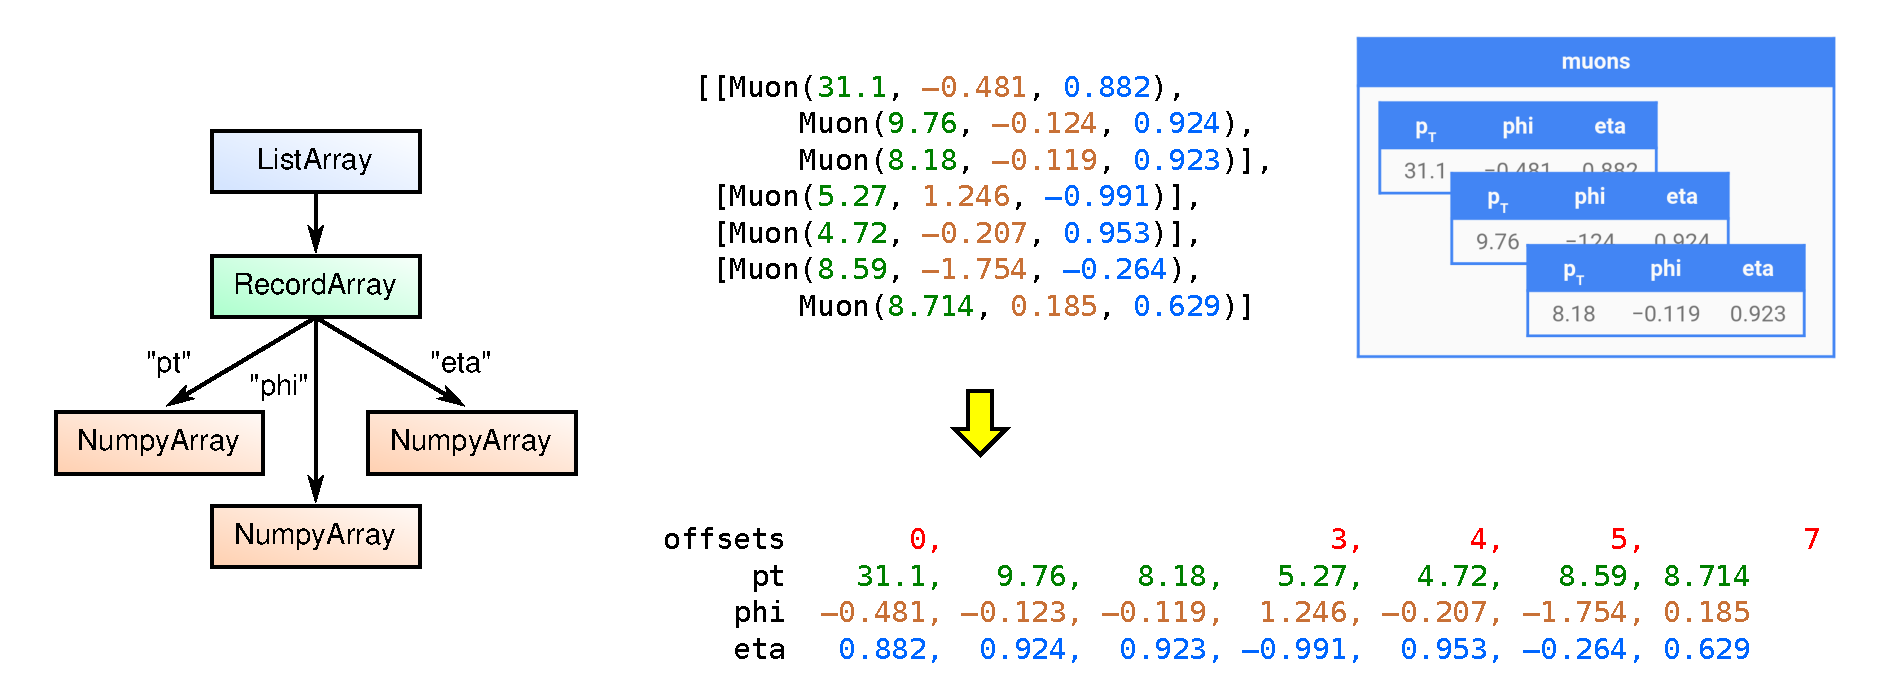
\includegraphics[width=\linewidth]{composable-3.pdf}}
\end{columns}
\end{frame}

\begin{frame}{\mbox{ }}
\vspace{0.5 cm}
\begin{center}

\includegraphics[width=0.5\linewidth]{awkward-logo.pdf}
\end{center}
\end{frame}

\begin{frame}{We now have 1 year of user feedback and maintainance experience}
\large
\vspace{0.5 cm}

\begin{columns}
\column{0.75\linewidth}
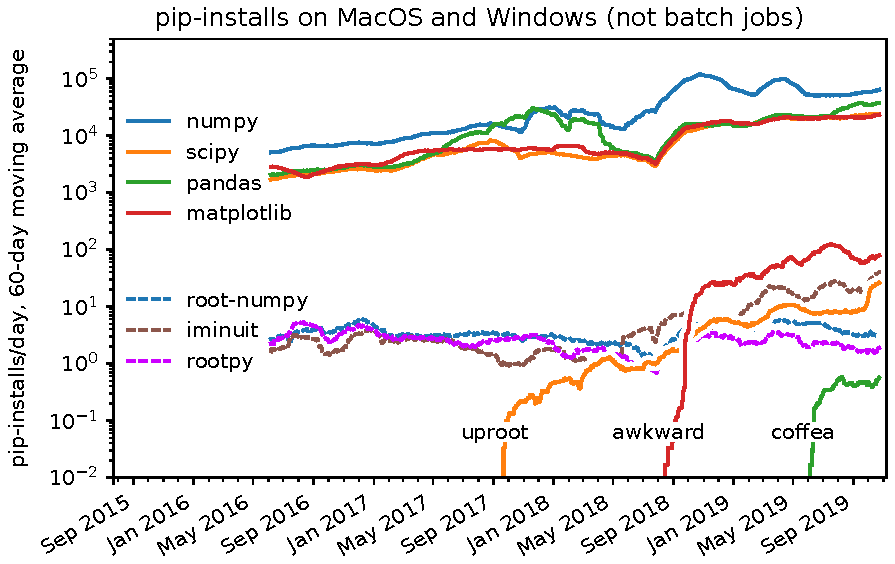
\includegraphics[width=\linewidth]{pip-timeline.pdf}

\vspace{0.1 cm}
\centering \textcolor{darkblue}{\fbox{awkward has 100 downloads/day, 2 issues/week}}

\column{0.3\linewidth}
\hfill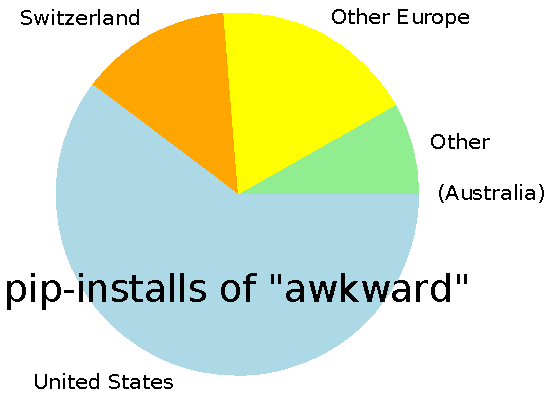
\includegraphics[width=0.8\linewidth]{pip-country-awkward.pdf}

\vspace{0.2 cm}
\hspace{-0.25 cm}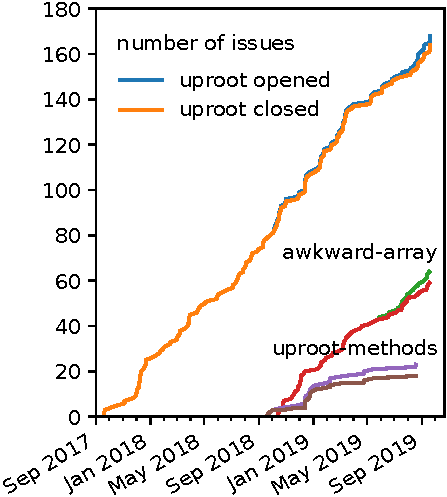
\includegraphics[width=\linewidth]{uproot-issues.pdf}
\end{columns}
\end{frame}

\begin{frame}{What I've learned}
\large
\vspace{0.5 cm}
\begin{block}{\Large From feedback and tutorials:}
\vspace{0.2 cm}
The interface needs to be simpler: a single \mintinline{python}{awkward.Array} class to hide the \mintinline{python}{ListArray} $\to$ \mintinline{python}{RecordArray} $\to$ \mintinline{python}{NumpyArrays} structure.

\vspace{0.2 cm}
Separate structural operations (e.g.\ cross-join) from physics (e.g.\ cross-product).
\end{block}

\vspace{0.5 cm}
\begin{uncoverenv}<2->
\begin{block}{\Large From maintenance:}
\vspace{0.2 cm}
Current implementation is entirely written in Python/Numpy.

\vspace{0.2 cm}
For better flexibility, robustness, and uniformity, and in a few cases, speed, it should be rewritten in C++.
\end{block}
\end{uncoverenv}
\end{frame}

\begin{frame}{New architecture}
\large
\vspace{0.5 cm}
\begin{columns}
\column{0.5\linewidth}
\vspace{-0.2 cm}

\textcolor{darkblue}{Layer 1:} Python user interface: a single \mintinline{python}{awkward.Array} class.
\vspace{\baselineskip}

\vspace{0.18 cm}
\textcolor{darkblue}{Layer 2:} Structural classes in Python

(e.g.\ \mintinline{python}{ListArray}/\mintinline{python}{RecordArray}).
\vspace{\baselineskip}

\vspace{0.18 cm}
\textcolor{darkblue}{Layer 3:} Array allocation and ownership; reference counting. Two languages: C++ and Numba (compiled Python).
\vspace{\baselineskip}

\vspace{0.18 cm}
\textcolor{darkblue}{Layer 4:} Implementations, where we write \mintinline{python}{for} loops. The only layer that needs to be optimized for speed.

\column{0.5\linewidth}
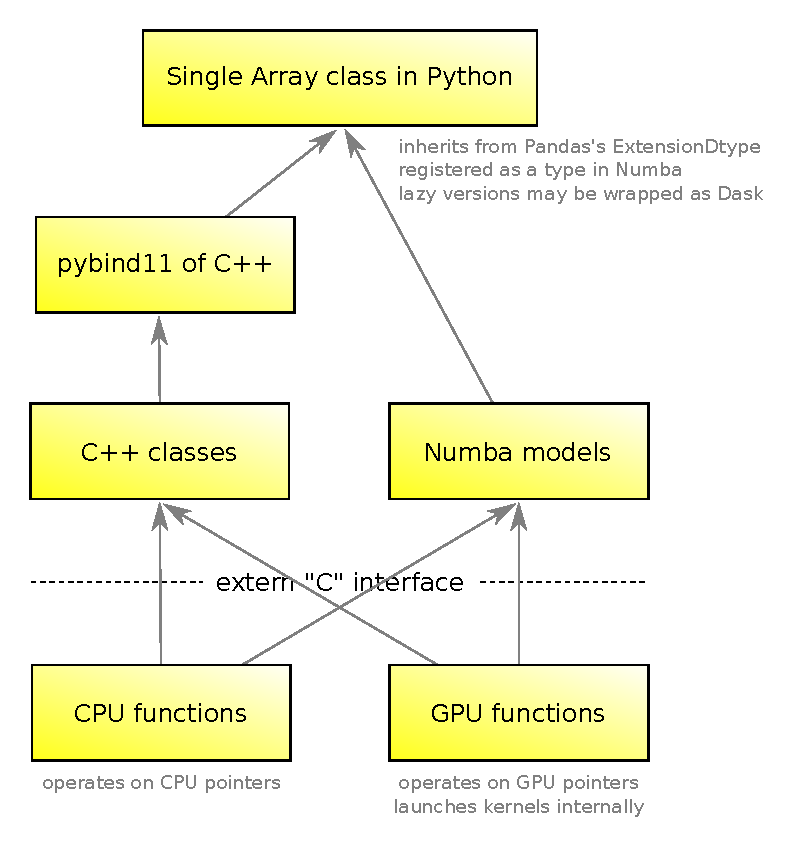
\includegraphics[width=\linewidth]{awkward-1-0-layers.pdf}
\end{columns}
\end{frame}



\end{document}
